\documentclass{standalone}
% translate with >> pdflatex -shell-escape <file>

% This file is an extract of the PGFPLOTS manual, copyright by Christian Feuersaenger.
% 
% Feel free to use it as long as you cite the pgfplots manual properly.
%
% See
%   http://pgfplots.sourceforge.net/pgfplots.pdf
% for the complete manual.
%
% Any required input files (for <plot table> or <plot file> or the table package) can be downloaded
% at
% http://www.ctan.org/tex-archive/graphics/pgf/contrib/pgfplots/doc/latex/
% and
% http://www.ctan.org/tex-archive/graphics/pgf/contrib/pgfplots/doc/latex/plotdata/

\usepackage{pgfplots}
\usepackage{pgfplotstable}
\pgfplotsset{compat=newest}

% The manual loads these libraries globally; the extracted standalone examples
% need them too. external/clickable/snakes are intentionally omitted.
\usetikzlibrary{
	arrows.meta,backgrounds,calc,decorations.footprints,decorations.markings,
	decorations.pathreplacing,fixedpointarithmetic,intersections,patterns,
	plotmarks,shapes.arrows,spy,through}
\usepgfplotslibrary{
	colorbrewer,colormaps,dateplot,fillbetween,groupplots,patchplots,polar,
	smithchart,statistics,ternary,units}

% Some colormap examples reuse this display style defined earlier in the manual.
\pgfplotsset{
	cycle from colormap manual style/.style={
		x=3cm,y=10pt,ytick=\empty,
		colorbar style={x=,y=,ytick=\empty},
		point meta min=0,point meta max=1,
		stack plots=y,
		y dir=reverse,colorbar style={y dir=reverse},
		every axis plot/.style={line width=2pt},
		legend entries={0,...,20},
		legend pos=outer north east,
	},
}

\pagestyle{empty}

\usepgfplotslibrary{fillbetween}

\begin{document}
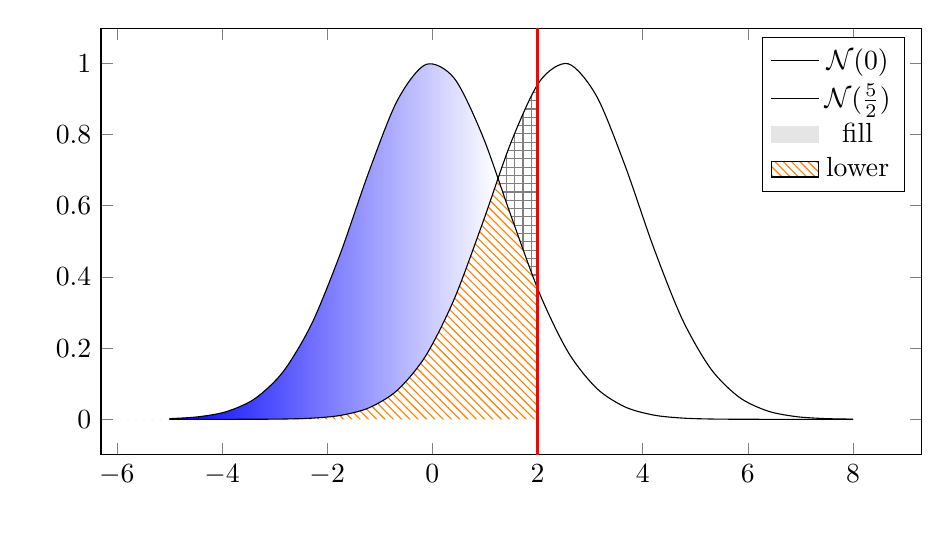
\begin{tikzpicture}

        \def\verticalbar{2}
    \begin{axis}[domain=-5:8,samples=25,smooth,width=12cm,height=7cm]
        % Draw curves
        \addplot [name path=g0,thin] {exp(-x^2/4)};
            \addlegendentry{$\mathcal{N}(0)$}
        \addplot [name path=g2.5,thin] {exp(-(x-2.5)^2/4)};
            \addlegendentry{$\mathcal{N}(\frac52)$}

        % Draw vertical bar:
        \draw [name path=red,red,thick]
            (\verticalbar,-1) -- (\verticalbar,2);

        \path [name path=axis] (-10,0) -- (16,0);

        \addplot [black!10] fill between [
            of=g0 and g2.5,
            soft clip={domain=-6:\verticalbar},
            split,
            every segment no 0/.style={left color=blue,right color=white},
            every segment no 1/.style={pattern=grid,pattern color=gray},
        ];
            \addlegendentry{fill}

        % compute + label the lower segment (but do not draw it):
        \path [name path=lower,
            %draw=red,ultra thick,
            intersection segments={of=g0 and g2.5,sequence=R1 -- L2}
        ];

        \addplot [pattern=north west lines, pattern color=orange]
            fill between [
                of=axis and lower,
                soft clip={domain=-6:\verticalbar},
        ];
            \addlegendentry{lower}
    \end{axis}
\end{tikzpicture}
\end{document}
